\documentclass[a4paper,12pt,oneside,pdflatex,italian,final,twocolumn]{article}

\usepackage[utf8]{inputenc}
\usepackage{parallel}
\usepackage{siunitx}
\usepackage{booktabs}
\usepackage{fancyhdr}
\usepackage{subcaption}
\usepackage{listings}
\usepackage{hyperref}

\usepackage[export]{adjustbox}
\usepackage[margin=0.5in]{geometry}
\addtolength{\topmargin}{0in}

\usepackage{libertine}
\renewcommand*\familydefault{\sfdefault}
\usepackage[T1]{fontenc}


\title{VIBIO Hardware Draft}
\author{Achmadi ST MT}
\date{Desember 2022}

\begin{document}

\pagestyle{fancy}

\lhead{VibrasticLab}
\chead{\today}
\rhead{Specification Document v1.0}

\onecolumn

\begin{figure}

\end{figure}\begin{minipage}{0.47\textwidth}
\centering

\end{minipage}
\hfill
\begin{minipage}{0.47\textwidth}
\raggedleft
\Huge \textbf{VIBIO Therapy Tools}
\end{minipage}

\section{Overview}

\begin{itemize}
    \item Intended  Hardware Port for Original VIBIO App

    \item Provides physical Push Button for actual interaction

    \item Based On RaspberryPi single board computer series equipped along with Touch LCD, Speaker, and Microphone

    \item The design currently in very early stage and not for end usage

\end{itemize}

\raggedright
\section{VIBIO App}

This is the original VIBIO App project preview:

\centering
\begin{figure} [h]
\centering
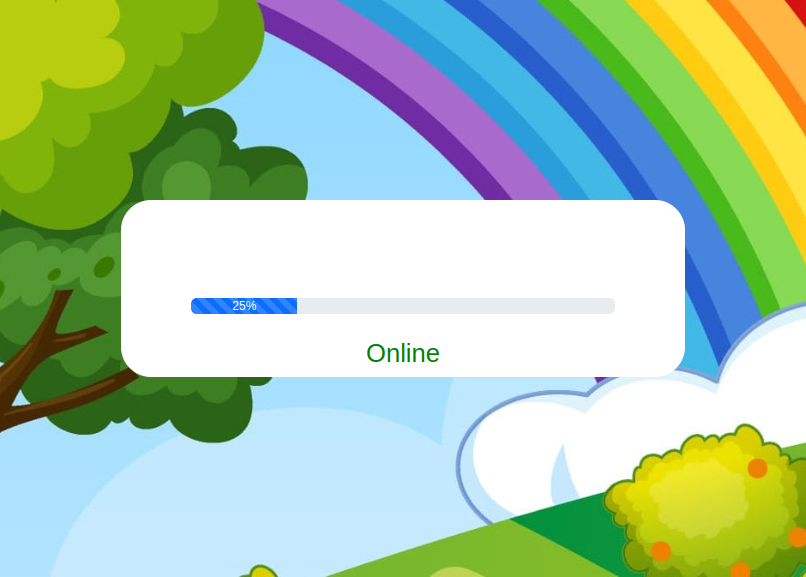
\includegraphics[width=0.8\textwidth,]{images/appstart.png}
\caption{VIBIO App prototype}
\end{figure}

\raggedright
Github Project Repository: \\
\url{https://github.com/mekatronik-achmadi/vibio}

\newpage
\section{Prototype Model}

Planned Prototype Design:

\centering
\begin{figure} [h]
\centering
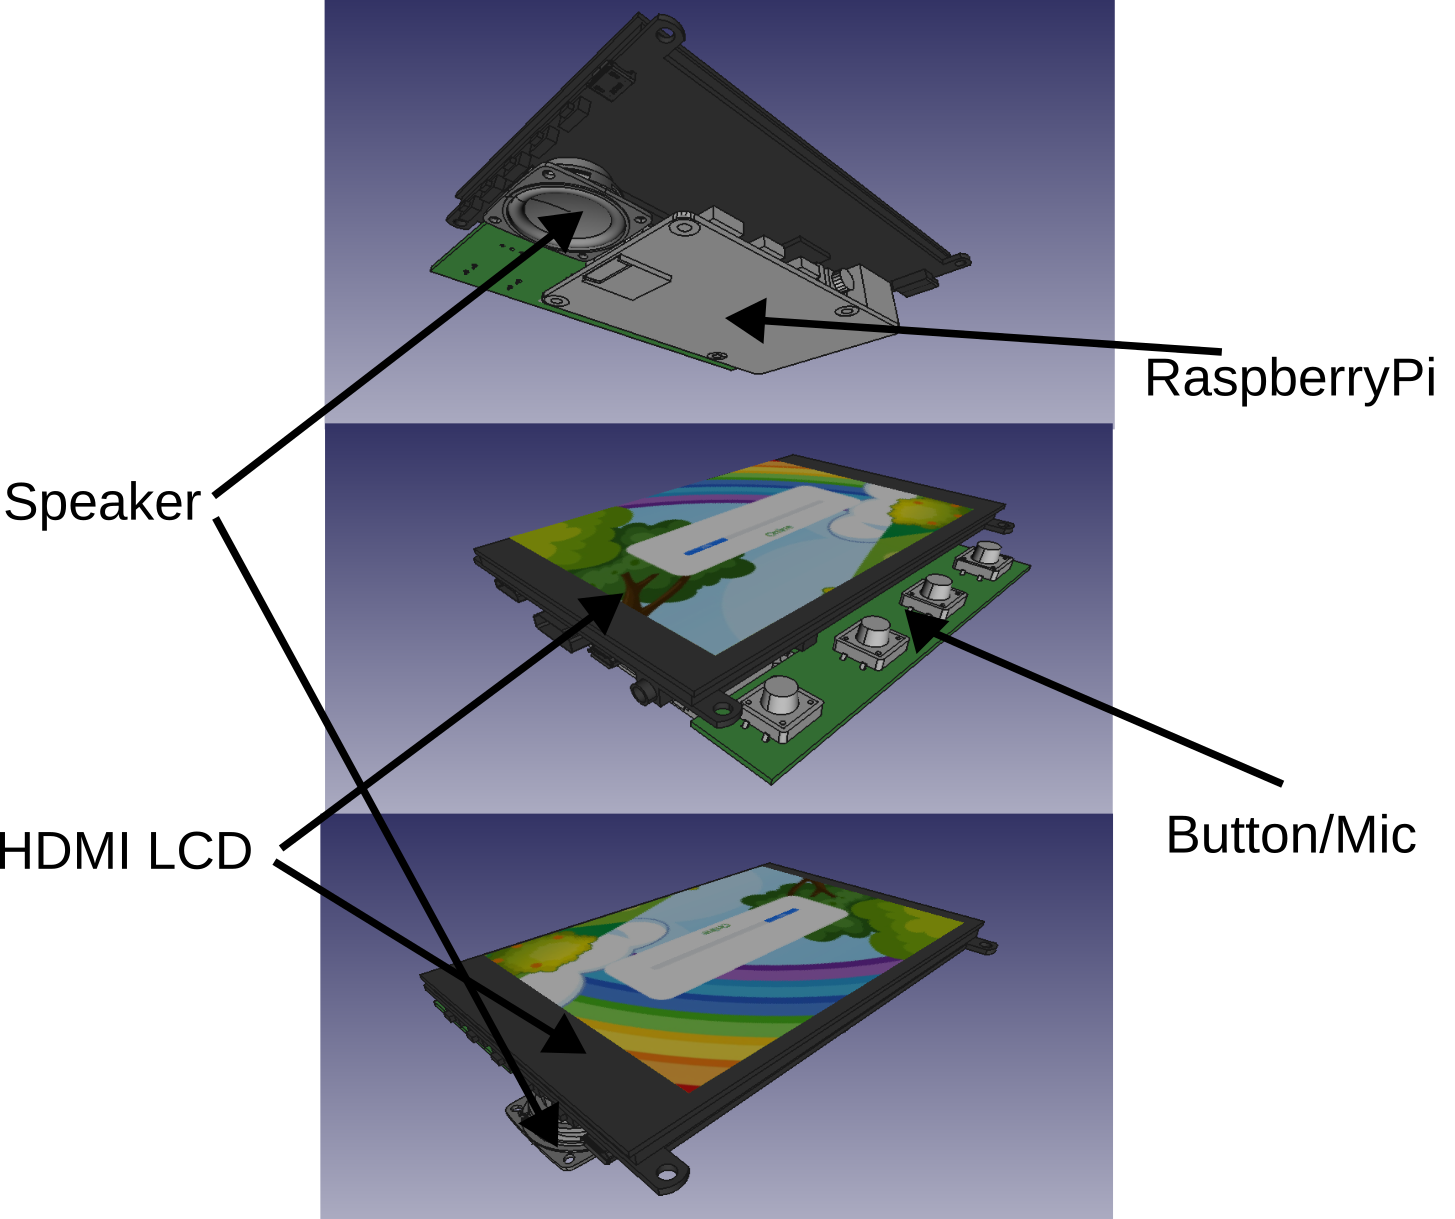
\includegraphics[width=\textwidth,]{images/proto.png}
\caption{Hardware Prototype}
\end{figure}

\raggedright
Github Project Repository:\\
\url{https://github.com/mekatronik-achmadi/short-jobs/tree/master/vibio/pcb-button}

\newpage
\section{Purchasing Estimation}

\subsection{Main Internal Components}

\centering
\begin{tabular}{|l|l|l|}
\toprule
Item & Price & URL \\
\midrule
RaspberryPi-3 & Rp. 1.259.000 & \href{https://www.tokopedia.com/libra-1/terbaru-raspberry-pi-3-model-b-1gb-ram-quad-core-1-2-ghz-with-wifi}{Tokopedia}  \\
Raspi LCD HDMI & Rp. 670.000 & \href{https://www.tokopedia.com/unorobotic/lcd-7-inci-raspberry-pi-ips-touchscreen-hdmi}{Tokopedia} \\
Speaker 3Inch & Rp. 130.000 & \href{https://www.tokopedia.com/jayaabadielectric/speaker-komponen-6-inch-lad-0806-original}{Tokopedia} \\
PCB Prototyping & Rp. 200.000 & \href{https://www.tokopedia.com/geraicerdas/cetak-pcb-1-keping-single-double-layer-rapid-prototyping-satuan}{Tokopedia} \\
Tombol+LED & Rp. 100.000 & Pasar Genteng Surabaya \\
Wire dkk & Rp. 200.000 & Pasar Genteng Surabaya \\
Ongkir Tokopedia & Rp. 100.000 & - \\
\midrule
Total & Rp. 2.659.000 & - \\
\bottomrule
\end{tabular}

\raggedright
\subsection{Packaging}

3D print Estimation: Rp. 2.000.000 (2000g)\\
\url{https://digiwarestore.com/en/appliances/3d-printer/}

\subsection{Total Per Unit}
Components + Packaging = Rp. 4.659.000
Round up for Accomodation = Rp. 5.000.000

\subsection{Development Task}
\begin{itemize}
    \item Main App Task: Mr Aprianto
    \item Hardware Implementation: Mr Achmadi
    \item Packaging Design: None
\end{itemize}

\end{document}
